\documentclass{ucll-slides}
\usepackage{pxfonts}
\usepackage{tikz}
\usepackage{calc}
\usepackage{ucll-code}


\usetikzlibrary{calc,shadows,tikzmark}
\usetikzlibrary{positioning}
\usetikzlibrary{shapes,snakes} 

\coursename{Distributed Applications}
\title{links and monitors}


\begin{document}

\maketitle

\section{Unlinked processes}

\begin{frame}
    \frametitle{2 processes (\&spawn/1)}
    \begin{center}
        
\begin{tikzpicture}[process/.style={circle,draw=green!60,fill=green!5,very thick, minimum size=7mm}]
            \coordinate (process A position) at (0,0);
            \coordinate (process B position) at ($ (process A position) + (2,0) $);
            \path[use as bounding box] ($ (process A position) + (-1,-1) $) rectangle ($ (process B position) + (1,1) $);

            \node[process] at (process A position) {A};
            \only<1>{
                \node[process] at (process B position) {B};
            }
            \only<2>{
                \node[cross out,draw] at (process B position) {B};
            }
        \end{tikzpicture}
    \end{center}
    \begin{overprint}
        \onslide<1>
        Two unlinked processes spawned

        \onslide<2>
        Process B dies

        \onslide<3>
        Process A keeps going
    \end{overprint}
\end{frame}













% ####################
% # LINKED PROCESSES #
% ####################
\section{Linked processes}

\begin{frame}
    \frametitle{2 processes (\&spawn\_link/1)}
    \begin{center}
        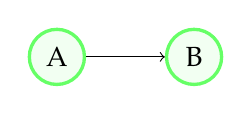
\begin{tikzpicture}[roundnode/.style={circle, draw=green!60, fill=green!5, very thick, minimum size=7mm}]
            %Nodes
            \node[roundnode]   (processA)                {A};
            \node[roundnode]   (processB)  [right=of processA]    {B};
            \draw[->] (processA.east) -- (processB.west);
        \end{tikzpicture}
    \end{center}
    Process A initiates link 
    \vfill
    (As process A:) \texttt{ProcessB |> Process.whereis |> Process.link}
\end{frame}

\begin{frame}
    \frametitle{2 processes (\&spawn\_link/1)}
    \begin{center}
        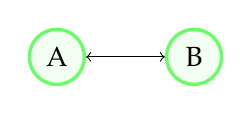
\begin{tikzpicture}[roundnode/.style={circle, draw=green!60, fill=green!5, very thick, minimum size=7mm}]
            %Nodes
            \node[roundnode]   (processA)                {A};
            \node[roundnode]   (processB)  [right=of processA]    {B};
            \draw[<->] (processA.east) -- (processB.west);
        \end{tikzpicture}
    \end{center}
    Processes are linked \textbf{bidirectionally}
\end{frame}

\begin{frame}
    \frametitle{2 processes (\&spawn\_link/1)}
    \begin{center}
        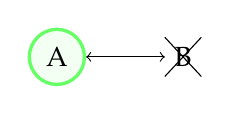
\begin{tikzpicture}[roundnode/.style={circle, draw=green!60, fill=green!5, very thick, minimum size=7mm}]
            \node[roundnode]   (processA)                {A};
            \node[cross out, draw]   (processB)  [right=of processA]    {B};
            \draw[<->] (processA.east) -- (processB.west);
        \end{tikzpicture}
    \end{center}

    Process B dies
\end{frame}

\begin{frame}
    \frametitle{2 processes (\&spawn\_link/1)}
    \begin{center}
        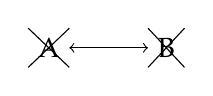
\begin{tikzpicture}[roundnode/.style={circle, draw=green!60, fill=green!5, very thick, minimum size=7mm}]
            \node[cross out, draw]   (processA)                {A};
            \node[cross out, draw]   (processB)  [right=of processA]    {B};
            \draw[<->] (processA.east) -- (processB.west);
        \end{tikzpicture}
    \end{center}

    Process A receives a "death message", and if it is not a system process, no custom behaviour can be implemented when this message is received.
    \vfill
    \textit{Note: Even if it is a system process, the end result should also be death. 
    This is often used when you want to do certain actions, such as cleaning up your process.}
\end{frame}











% ############
% # MONITORS #
% ############
\section{Monitors}

\begin{frame}
    \frametitle{2 processes (\&spawn/1)}
    \begin{center}
        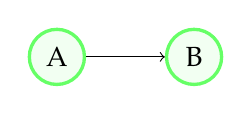
\begin{tikzpicture}[roundnode/.style={circle, draw=green!60, fill=green!5, very thick, minimum size=7mm}]
            \node[roundnode]   (processA)                {A};
            \node[roundnode]   (processB)  [right=of processA]    {B};
            \draw[->] (processA.east) -- (processB.west);
        \end{tikzpicture}
    \end{center}
    Process A initiates monitoring
    \vfill
    ProcessB $|>$ Process.whereis $|>$ Process.monitor
\end{frame}

\begin{frame}
    \frametitle{2 processes (\&spawn/1)}
    \begin{center}
        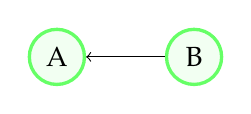
\begin{tikzpicture}[roundnode/.style={circle, draw=green!60, fill=green!5, very thick, minimum size=7mm}]
            \node[roundnode]   (processA)                {A};
            \node[roundnode]   (processB)  [right=of processA]    {B};
            \draw[<-] (processA.east) -- (processB.west);
        \end{tikzpicture}
    \end{center}
    Processes are linked \textbf{unidirectionally}
\end{frame}

\begin{frame}
    \frametitle{2 processes (\&spawn/1)}
    \begin{center}
        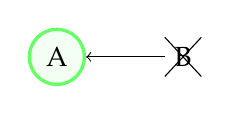
\begin{tikzpicture}[roundnode/.style={circle, draw=green!60, fill=green!5, very thick, minimum size=7mm}]
            \node[roundnode]   (processA)                {A};
            \node[cross out, draw]   (processB)  [right=of processA]    {B};
            \draw[<-] (processA.east) -- (processB.west);
        \end{tikzpicture}
    \end{center}

    Process B dies
    \vfill
    When something happens to B, A will receive a message.
\end{frame}

\begin{frame}
    \frametitle{2 processes (\&spawn/1)}
    \begin{center}
        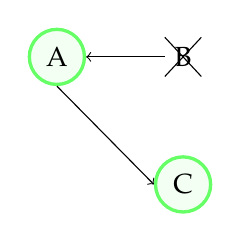
\begin{tikzpicture}[roundnode/.style={circle, draw=green!60, fill=green!5, very thick, minimum size=7mm}]
            \node[roundnode]   (processA)                {A};
            \node[cross out, draw]   (processB)  [right=of processA]    {B};
            \node[roundnode]   (processC)  [below=of processB]    {C};
            \draw[<-] (processA.east) -- (processB.west);
            \draw[->] (processA.south) -- (processC.west);
        \end{tikzpicture}
    \end{center}
    \vfill
    Process A receives a "death message". A sample usage of a monitoring process would be starting up another process.
\end{frame}

\end{document}
